\begin{figure}
	\centering
	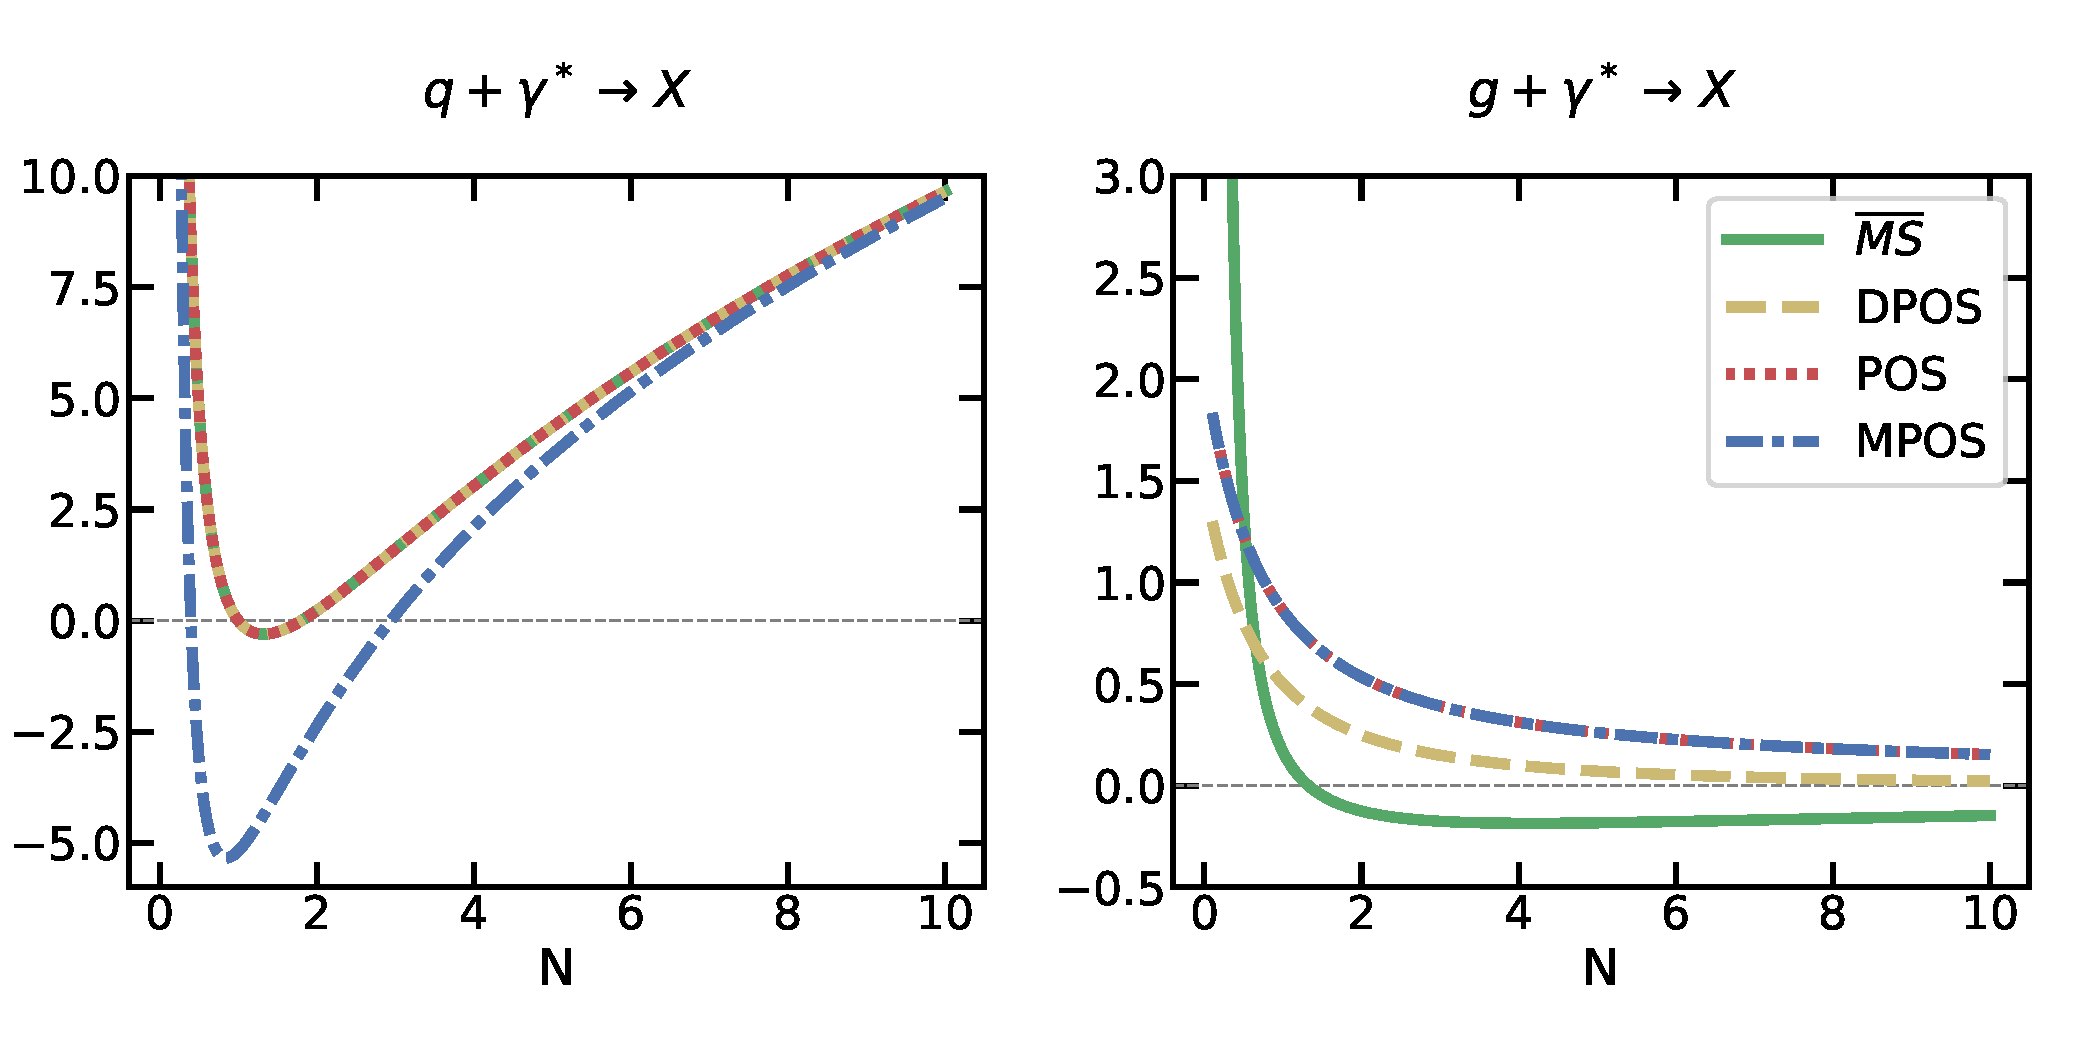
\includegraphics[width=0.7\textwidth]{ch-qcd/dis}
\end{figure}

The Deep Inelastic Scattering process is the scattering of a lepton over an
hadron component, mediated by an |EW| boson.

The leptonic part does not couple directly to |QCD|, thus the :math:`\alpha_s`
corrections do apply only to the hadronic side (at |LO| |EW|), and the |EW|
boson can be seen as emitted from the incoming lepton and absorbed into the
hadron.

In this picture the process can be interpreted as the scattering of an off-shell
|EW| boson over an hadron, probing the hadron composition.
